\documentclass[11pt,a4paper]{article}
\usepackage[margin=2.3cm]{geometry}
\usepackage[T1]{fontenc}
\usepackage{lmodern}
\usepackage{microtype}
\usepackage{amsmath}
\usepackage{booktabs}
\usepackage{longtable}
\usepackage{tabularx}
\usepackage{graphicx}
\usepackage{xcolor}
\usepackage{caption}
\usepackage{enumitem}
\usepackage{algorithm}
\usepackage{algpseudocode}
\usepackage{tikz}
\usetikzlibrary{positioning,arrows.meta,fit,backgrounds}
\usepackage[hidelinks]{hyperref}

\definecolor{ink2}{HTML}{52514E}
\definecolor{aseq}{HTML}{2A78D6}
\definecolor{boxbg}{HTML}{F3F7FD}
\definecolor{warnbg}{HTML}{FFF6E0}

\captionsetup{font=small,labelfont=bf,width=0.95\linewidth}
\setlist{itemsep=2pt,topsep=3pt}
\newcommand{\code}[1]{\texttt{#1}}
\newcommand{\figref}[1]{Fig.~\ref{#1}}
\newcommand{\tabref}[1]{Table~\ref{#1}}
\newcommand{\secref}[1]{Section~\ref{#1}}

\setlength{\emergencystretch}{2.5em}
\renewcommand{\topfraction}{0.9}
\renewcommand{\bottomfraction}{0.8}
\renewcommand{\textfraction}{0.07}
\renewcommand{\floatpagefraction}{0.75}
\setcounter{totalnumber}{4}
% generated by make_figures.py; do not edit
\newcommand{\chAseqRows}{20}
\newcommand{\chAseqShort}{4}
\newcommand{\chAseqSilent}{0}
\newcommand{\chAseqUnverified}{0}
\newcommand{\chBBestOther}{Kingfisher 0.5.0}
\newcommand{\chBBestOtherMed}{1,715}
\newcommand{\chBDefConn}{21.7}
\newcommand{\chBDefMBps}{10.1}
\newcommand{\chBDefMax}{3,789}
\newcommand{\chBDefMed}{2,561}
\newcommand{\chBDefMin}{850}
\newcommand{\chBDefRatioMed}{1.96}
\newcommand{\chBDefVsBestOther}{5.8}
\newcommand{\chBDefVsBestOtherMin}{0.3}
\newcommand{\chBFixConn}{23.8}
\newcommand{\chBFixMBps}{37.0}
\newcommand{\chBFixMax}{1,307}
\newcommand{\chBFixMed}{699}
\newcommand{\chBFixMin}{323}
\newcommand{\chBFixVsBestOther}{7.6}
\newcommand{\chBOtherMBpsMax}{5.4}
\newcommand{\chBTimeouts}{4}
\newcommand{\chBWorstOtherMed}{30,000}
\newcommand{\chOtherRows}{40}
\newcommand{\chOtherSilent}{8}
\newcommand{\chOtherTimeouts}{10}
\newcommand{\chOtherUnverified}{204}
\newcommand{\chRBestOther}{Kingfisher 0.5.0}
\newcommand{\chRBestOtherMed}{5,825}
\newcommand{\chRDefConn}{15.6}
\newcommand{\chRDefMBps}{8.9}
\newcommand{\chRDefMax}{2,927}
\newcommand{\chRDefMed}{855}
\newcommand{\chRDefMin}{826}
\newcommand{\chRDefRatioMed}{1.60}
\newcommand{\chRDefVsBestOther}{6.1}
\newcommand{\chRDefVsBestOtherMin}{3.2}
\newcommand{\chRFixConn}{15.6}
\newcommand{\chRFixMBps}{9.5}
\newcommand{\chRFixMax}{1,317}
\newcommand{\chRFixMed}{794}
\newcommand{\chRFixMin}{242}
\newcommand{\chRFixVsBestOther}{9.8}
\newcommand{\chROtherMBpsMax}{1.3}
\newcommand{\chRTimeouts}{6}
\newcommand{\chRWorstOtherMed}{10,223}
\newcommand{\chainEnd}{Nov 1}
\newcommand{\chainStart}{Oct 26}
\newcommand{\distinctWinners}{7}
\newcommand{\mdBCases}{27}
\newcommand{\mdBRows}{48}
\newcommand{\mdCases}{44}
\newcommand{\mdRows}{96}
\newcommand{\mdTotal}{178}
\newcommand{\noiseArms}{2.09}
\newcommand{\noiseReps}{1.53}
\newcommand{\noiseRepsMax}{12.7}
\newcommand{\panelsChangingWinner}{5}
\newcommand{\portalDays}{17}
\newcommand{\portalEmpty}{7}
\newcommand{\portalEnd}{Nov 1}
\newcommand{\portalFail}{107}
\newcommand{\portalFailPct}{3.1}
\newcommand{\portalFiveHundred}{80}
\newcommand{\portalMaxS}{59}
\newcommand{\portalMedianS}{0.82}
\newcommand{\portalProbes}{3,420}
\newcommand{\portalSlow}{212}
\newcommand{\portalStart}{Oct 15}
\newcommand{\portalTimeout}{27}
\newcommand{\probeN}{38}
\newcommand{\probeOneMax}{7.2}
\newcommand{\probeOneMed}{2.0}
\newcommand{\probeOneMin}{0.5}
\newcommand{\probeScaleMed}{18.4}
\newcommand{\probeTwentyMax}{99.7}
\newcommand{\probeTwentyMed}{36.2}
\newcommand{\probeTwentyMin}{0.0}
\newcommand{\rtBoConn}{13.9}
\newcommand{\rtBoRatio}{1.62}
\newcommand{\rtBoWins}{4}
\newcommand{\rtBoWorst}{3.80}
\newcommand{\rtBuConn}{13.1}
\newcommand{\rtBuRatio}{1.84}
\newcommand{\rtBuWins}{4}
\newcommand{\rtBuWorst}{3.93}
\newcommand{\rtGrConn}{20.8}
\newcommand{\rtGrRatio}{1.41}
\newcommand{\rtGrWins}{6}
\newcommand{\rtGrWorst}{3.80}
\newcommand{\rtJsfConn}{20.4}
\newcommand{\rtJsfRatio}{1.35}
\newcommand{\rtJsfWins}{9}
\newcommand{\rtJsfWorst}{2.91}
\newcommand{\rtJtwConn}{19.2}
\newcommand{\rtJtwRatio}{1.55}
\newcommand{\rtJtwWins}{7}
\newcommand{\rtJtwWorst}{3.81}
\newcommand{\rtKnConn}{12.8}
\newcommand{\rtKnRatio}{2.15}
\newcommand{\rtKnWins}{5}
\newcommand{\rtKnWorst}{10.04}
\newcommand{\rtTdConn}{18.9}
\newcommand{\rtTdRatio}{1.39}
\newcommand{\rtTdWins}{3}
\newcommand{\rtTdWorst}{3.80}
\newcommand{\sweepBBest}{428}
\newcommand{\sweepBBestJ}{64}
\newcommand{\sweepBDefault}{581}
\newcommand{\sweepBEight}{731}
\newcommand{\sweepBOne}{9,708}
\newcommand{\sweepBSpeedup}{23}
\newcommand{\sweepRBest}{271}
\newcommand{\sweepRBestJ}{32}
\newcommand{\sweepRDefault}{447}
\newcommand{\sweepREight}{522}
\newcommand{\sweepROne}{4,197}
\newcommand{\sweepRSpeedup}{15}
\newcommand{\varBFold}{39}
\newcommand{\varBMax}{80.0}
\newcommand{\varBMin}{2.1}
\newcommand{\varBN}{14}
\newcommand{\varRFold}{5}
\newcommand{\varRMax}{31.3}
\newcommand{\varRMin}{5.8}
\newcommand{\varRN}{14}
\newcommand{\verFirstMed}{6,552}
\newcommand{\verGain}{2.6}
\newcommand{\verLastMed}{2,561}


\title{\textbf{adaptiSeq: problem, design and evaluation}\\[2pt]
\large Methodology and evaluation material for a paper on parallel, verified download of public sequencing data}
\author{Draft generated from the benchmark record, \today}
\date{}

\begin{document}
\maketitle

\begin{abstract}
\noindent
Downloading a list of public sequencing runs is a routine first step of genomics work, and on today's
archives it is slow and unreliable. The European Nucleotide Archive (ENA) limits each TCP connection to
a few megabytes per second, its metadata service fails for hours at a time, and it sometimes serves a
file whose bytes do not match its own checksum. Tools that fetch one file at a time over one connection
take hours for a list that the link could carry in minutes, and when the archive misbehaves they often
finish with exit status 0 while runs are missing or were silently fetched from another archive.
adaptiSeq is a Python downloader built for this setting. It splits files into byte ranges fetched over
many connections, keeps those connections busy until the last byte, treats a refused connection as a
ceiling rather than as distress, checks every file against the archive's md5 as it lands and re-fetches a
bad copy in parallel, and fails loudly instead of substituting or skipping. This document describes the
problem, each design decision and the measurement that motivated it, and an evaluation on SDSC Expanse
spanning \portalDays{} days of archive monitoring and six benchmark campaigns. On a 241-run ENA list the fastest
other tool that downloaded every run was, in the median repetition, \chRDefVsBestOther{} times slower than adaptiSeq's
default and \chRFixVsBestOther{} times slower than its fixed pool, and in \chAseqRows{} benchmark rows it never exited 0 with a run missing, against \chOtherSilent{} of
\chOtherRows{} rows for iSeq, Kingfisher and fastq-dl. We also report where the design does not win: a
fixed worker count was faster than the adaptive default on most ENA cases, and every result depends on the
state of ENA's and NCBI's servers during the run.
\end{abstract}

\tableofcontents
\newpage

%=====================================================================
\section{The problem}
\label{sec:problem}
%=====================================================================

\subsection{The task}
A study, a meta-analysis or a pipeline starts from a list of accessions: projects, samples, experiments or
runs in ENA, NCBI's Sequence Read Archive (SRA), DDBJ, GEO or China's Genome Sequence Archive (GSA). Each
accession resolves to one or more runs, and each run to one to three FASTQ files (single-end, paired-end,
or paired-end plus an unpaired or barcode file). The archives publish an md5 checksum for every FASTQ
file. The job is to obtain every file of every run, byte-identical to the archive's copy, as fast as the
network allows, and to report exactly which runs could not be obtained.

Two list shapes dominate in practice and stress a downloader differently:
\begin{itemize}
\item \textbf{Many small runs.} Our list D1 has 241 runs, 321 files and 7.6~GB (mean 24~MB per file; 40 runs
have three files). Per-file overhead (metadata query, connection setup, md5) is a large share of the work, so
a tool must keep many files in flight.
\item \textbf{Few large runs.} Our list D2 has 8 runs, 16 files and 25.9~GB (1.4 to 1.9~GB per file). There are
too few files to fill the link one file per connection, so a tool must split each file across connections.
\end{itemize}

\subsection{What makes it hard: the archives}
\label{sec:archives}
We measured the archives throughout the work (\secref{sec:method}). Five properties shape the design.

\paragraph{P1. Throughput is per connection.} ENA serves each TCP connection at roughly \probeOneMed{}~MB/s
(median of \probeN{} probes from Expanse compute nodes, range \probeOneMin{} to \probeOneMax{}~MB/s), and the
aggregate grows almost linearly with the number of parallel connections: the median job got \probeTwentyMed{}~MB/s
with 20 connections, \probeScaleMed{} times its single-connection rate (\figref{fig:probe}). A tool that uses one
connection per file therefore leaves most of the path idle, whatever the network.

\begin{figure}[!htb]
\centering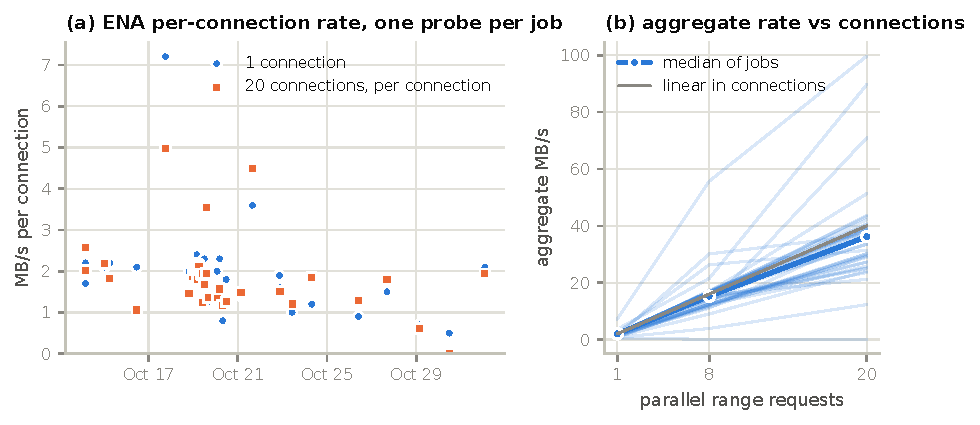
\includegraphics[width=\linewidth]{figs/link_probe.pdf}
\caption{ENA's per-connection rate. Each benchmark job started with a 20-second probe of 1, 8 and 20 parallel
HTTPS range requests to one ENA file from the compute node. (a) Per-connection rate by date: around 2~MB/s, with
days at 0.5 and at 7~MB/s. (b) Aggregate rate against connections (one faint line per job): close to linear up
to 20 connections, so parallelism is the only lever a client has. One job (Oct 30) saw near-zero rates at 8 and
20 connections while single connections still moved data.}
\label{fig:probe}
\end{figure}

\paragraph{P2. The archive's state changes by the hour.} The per-connection rate in \figref{fig:probe}a varies
more than tenfold between days. ENA's metadata service is less stable still. We queried its \code{filereport}
API every 5 minutes for \portalDays{} days (\portalStart{} to \portalEnd{}, \portalProbes{} queries; \figref{fig:portal}):
\portalFail{} queries (\portalFailPct\%) failed outright with HTTP~500 (\portalFiveHundred) or no answer within
60~s (\portalTimeout), \portalSlow{} more took over 10~s to answer, and \portalEmpty{} came back as HTTP~200 with no
rows for a run that exists. Failures cluster into episodes of hours (Oct 15--16, Oct 19--21, Oct 31). During such an
episode every tool that relies on the API is affected, and a benchmark arm that happens to run then measures the
episode, not the tool.

\begin{figure}[!htb]
\centering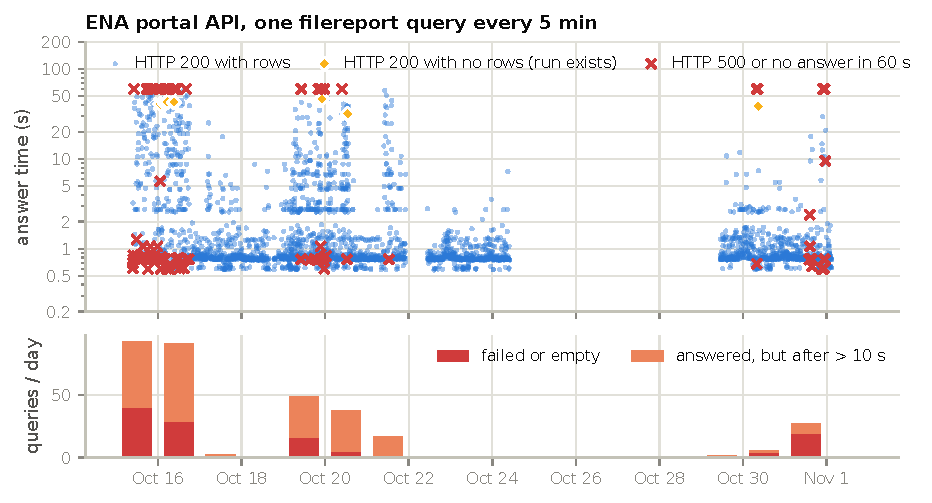
\includegraphics[width=\linewidth]{figs/portal.pdf}
\caption{ENA's portal API over \portalDays{} days. Top: answer time of each query (log scale); crosses are HTTP~500
or no answer in 60~s, diamonds are HTTP~200 with no rows for a run that is in ENA. Bottom: failed or empty answers
and slow answers per day. The gap from Oct 24 to Oct 29 is a pause in the monitor, not in the service. The
median successful answer took \portalMedianS{}~s; the slowest took \portalMaxS{}~s.}
\label{fig:portal}
\end{figure}

\paragraph{P3. The archive sometimes serves bad bytes.} We counted \mdTotal{} md5 mismatches in the logs of the
\mdRows{} benchmark rows of the two main campaigns, in \mdCases{} of the rows (\figref{fig:md5}). They hit every
tool, they land on different files in different arms of the same hour, and a plain \code{curl} over FTP produced a
file of exactly the right length with the wrong md5 (diagnostic job \code{55055531}). The same file can be bad for
hours: \code{SRR22904330\_1} failed md5 in two tools on Oct 27 and was fetched cleanly by every adaptiSeq arm the day
before. A downloader cannot prevent this; it can only detect it and fetch again.

\paragraph{P4. The archive refuses and cuts connections.} ENA accepts about 25 simultaneous connections from one
client and refuses further connects; the ceiling moves (we saw 25 on some days and 50 on others). It also ends some
responses short of their \code{Content-Length}, answers some range requests with 403 or 416, and resets FTP data
connections under load. GSA cuts streams at any load (hundreds of cut responses per panel in round 3). A client that
reads each of these as ``the server is overloaded'' backs off to a few connections and stays there.

\paragraph{P5. Failure is easy to hide.} When ENA's API fails, the common response is to assume the run is not in ENA
and fetch the \code{.sra} file from NCBI instead, then convert it to FASTQ. The converted file cannot be checked
against ENA's md5, and the tool still reports success. Other tools stop at the first corrupt file, or give up on a run
after retries, and still exit 0. A user who trusts the exit status gets an incomplete or unverifiable data set
without being told (\secref{sec:complete}).

\subsection{Requirements}
\label{sec:req}
From P1 to P5 we derived the requirements in \tabref{tab:req}. Each is met by one or more mechanisms in
\secref{sec:design} and checked by a measurement in \secref{sec:eval}.

\begin{table}[h]
\centering\small
\begin{tabularx}{\linewidth}{@{}l X X l@{}}
\toprule
 & Requirement & Mechanism (\secref{sec:design}) & Evidence \\
\midrule
R1 & Use many connections at once, across files and within a file & batch pool; segmented ranges & \figref{fig:jsweep} \\
R2 & Keep connections busy until the last byte & work stealing; tail and spare-budget splits & \figref{fig:tail}, \ref{fig:versions} \\
R3 & Treat refusals at a ceiling as a limit, not as distress & per-host guard: hold, wait, recover & \figref{fig:versions} \\
R4 & Check every file and re-fetch bad copies without stalling the list & in-pool md5, re-queue & \figref{fig:md5}, \ref{fig:complete} \\
R5 & Never substitute or skip silently; fail with a non-zero exit & ENA patience; announced fallback; \code{fail.log} & \figref{fig:complete} \\
R6 & Work without per-list tuning, on every archive & adaptive controller; HTTPS-first transport & \figref{fig:r3heat}, \ref{fig:r3conn} \\
R7 & Survive interruption & \code{.part} + \code{.part.meta} resume & \secref{sec:engine} \\
R8 & Be usable from code, not only the shell & Python API, typed errors & \secref{sec:api} \\
\bottomrule
\end{tabularx}
\caption{Requirements, the mechanisms that address them, and where they are evaluated.}
\label{tab:req}
\end{table}

%=====================================================================
\section{Design}
\label{sec:design}
%=====================================================================

\subsection{Overview}
adaptiSeq (version 0.1.12 throughout this document) keeps iSeq's command line and its accession, metadata,
integrity and merge behaviour~\cite{iseq}, reimplemented in Python, and replaces the transfer path. All sequence
bytes pass through one download seam, so the scheduler and engine change \emph{how} and \emph{when} bytes arrive,
never \emph{which} bytes. \figref{fig:arch} shows the path of a list.

\begin{figure}[!htb]
\centering
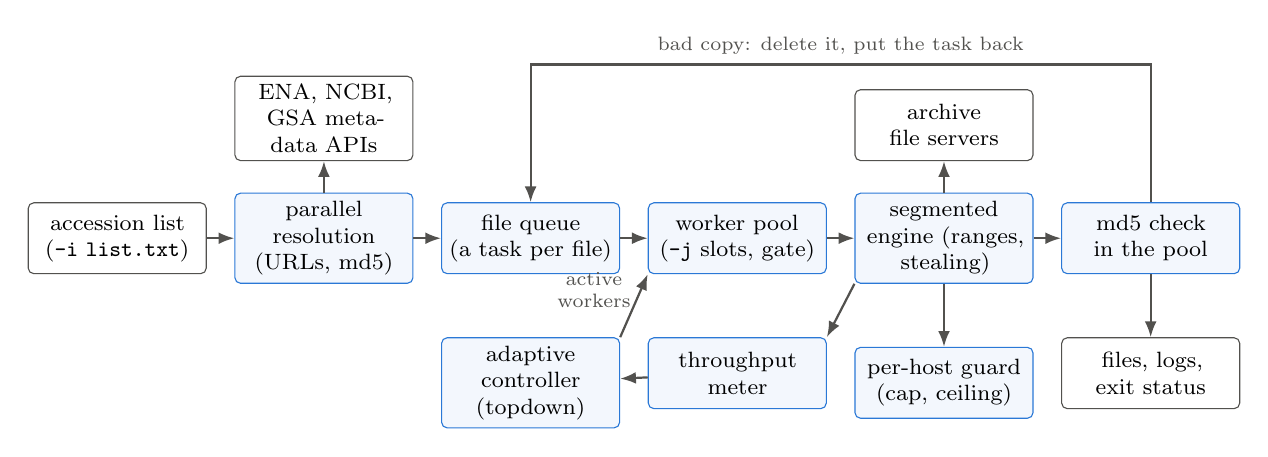
\begin{tikzpicture}[
  node distance=4mm and 3.5mm,
  box/.style={draw=aseq, fill=boxbg, rounded corners=2pt, align=center, font=\footnotesize, inner sep=3pt,
              minimum height=9mm, text width=2.05cm},
  ext/.style={draw=ink2, fill=white, rounded corners=2pt, align=center, font=\footnotesize, inner sep=3pt,
              minimum height=9mm, text width=2.05cm},
  arr/.style={-{Latex[length=2mm]}, draw=ink2, thick},
  lab/.style={font=\scriptsize, text=ink2, align=center}]
\node[ext] (list) {accession list\\(\code{-i list.txt})};
\node[box, right=of list] (res) {parallel resolution (URLs, md5)};
\node[box, right=of res] (queue) {file queue\\(a task per file)};
\node[box, right=of queue] (pool) {worker pool\\(\code{-j} slots, gate)};
\node[box, right=of pool] (eng) {segmented engine (ranges, stealing)};
\node[box, right=of eng] (ver) {md5 check in the pool};
\node[ext, above=of res] (api) {ENA, NCBI, GSA metadata APIs};
\node[ext, above=of eng] (arch) {archive file servers};
\node[box, below=8mm of queue] (ctrl) {adaptive controller (topdown)};
\node[box, below=8mm of pool] (meter) {throughput meter};
\node[box, below=8mm of eng] (guard) {per-host guard (cap, ceiling)};
\node[ext, below=8mm of ver] (out) {files, logs, exit status};
\draw[arr] (list) -- (res);
\draw[arr] (res) -- (api);
\draw[arr] (res) -- (queue);
\draw[arr] (queue) -- (pool);
\draw[arr] (pool) -- (eng);
\draw[arr] (eng) -- (arch);
\draw[arr] (eng) -- (ver);
\draw[arr] (ver) -- (out);
\draw[arr] (eng) -- (guard);
\draw[arr] (eng.south west) -- (meter.north east);
\draw[arr] (meter) -- (ctrl);
\draw[arr] (ctrl.north east) -- node[lab, left, pos=0.75]{active\\workers} (pool.south west);
\draw[arr] (ver.north) |- ++(0,1.75) -| node[lab, above, pos=0.25]{bad copy: delete it, put the task back} (queue.north);
\end{tikzpicture}
\caption{The path of an accession list through adaptiSeq. Resolution runs in parallel under per-archive request
limits. Each file becomes a task; a pool of workers takes tasks, the engine splits each file into byte ranges on
several connections, a per-host guard bounds the connections and reacts to refusals, and each finished file is
md5-checked inside the pool. A bad copy goes back to the queue. The controller reads the byte rate and sets how
many workers may start files.}
\label{fig:arch}
\end{figure}

\subsection{Resolution and metadata under an unreliable API}
\label{sec:resolve}
\textbf{Parallel, rate-limited resolution.} Accessions are resolved concurrently (\code{-{}-meta-jobs}, default 3)
under per-endpoint token buckets: 8 requests/s for ENA, 5 for GSA, 3 for NCBI (10 with an API key). Resolution
yields, for each file, its URL, size and the archive's md5.

\textbf{Telling ``failed'' from ``not there''.} ENA's API fails in ways that look like an answer (P2): HTTP~500 with
an HTML page, an in-band \code{ERROR occurred} line under HTTP~200, an empty body, or an empty table after a long
wait. Early versions, like iSeq, read any of these as ``this run is not in ENA'' and fell back to SRA; in the 0.1.4
benchmark, one ENA outage turned an entire adaptiSeq arm into SRA downloads (0 of 241 runs verifiable against ENA).
adaptiSeq now retries a failed query with backoff (2, 4, 8, 16, then 30~s apart), counts an empty answer that took
more than 5~s as a failure, and allows up to 3 minutes of continuous portal failure before it falls back. The 3
minutes are shared by all accessions of a list, so an outage costs a list about 3 minutes, not 3 minutes per run.

\textbf{Fallback is announced, and can be refused.} When a run really has no usable ENA record, adaptiSeq says which
accessions it will fetch from SRA and records that they are not md5-verified; \code{-{}-no-sra-fallback} turns the
fallback into a failure, so every kept file is verified against ENA.

\textbf{A GSA run missing from GSA's table fails.} GSA's run-info table occasionally omits a run. adaptiSeq retries
the query and, if the run is still absent, fails the accession with a non-zero exit, instead of printing ``finished''
for a run that downloaded nothing (an adaptiSeq bug found in round 2, fixed in 0.1.12).

\subsection{Transport selection}
For ENA, whose files are reachable over FTP and HTTPS on the same host, adaptiSeq prefers HTTPS: it probes the host
once with a range request and, if ranges are honoured, uses segmented HTTPS for every file on that host. Otherwise
it uses segmented FTP (\code{REST}/\code{RETR}), then a single stream. The probe takes a connection slot like any
segment, waits at the connection ceiling, and is retried up to 4 times; an unanswered probe used to be read as ``no
range support'', which sent 1.5--2~GB files down one connection for 15--30 minutes each (0.1.6). The verdict is cached
per host, by kind, not URL. \emph{Limitation:} because the verdict is cached for the whole list, one probe that fails
for a transient reason sends the whole list to FTP, which ENA serves poorly under load (\secref{sec:adaptive}).

\subsection{The segmented engine}
\label{sec:engine}
The engine is ported from FastBioDL~\cite{fastbiodl} and extended. A file of size $S$ is planned as
\[ n(S) = \min\bigl(8,\ \max(1, \lfloor S / 512\,\text{MiB}\rfloor)\bigr) \]
byte ranges (files under 5~MiB use one), each fetched on its own connection with a strict \code{206 Partial Content} check and written in place with \code{pwrite}. Progress is
recorded in a \code{.part.meta} file, so an interrupted download resumes per range (R7), and a resume state whose
\code{.part} data is missing is discarded rather than trusted (an early bug left zero-filled regions).

Three mechanisms keep connections busy until the end of a file (R2):
\begin{enumerate}
\item \textbf{Work stealing.} When a range finishes, its connection takes the second half of the largest remaining
range of the same file, if each half is at least 16~MiB. Without it, the last bytes of each file arrived on one
connection while the others sat idle; on D2 that tail took 15 of 26 minutes (0.1.5 trace, job \code{55061744}).
\item \textbf{Tail splitting.} A file that starts near the end of a list, or is re-fetched after an md5 mismatch,
gets $\lfloor \text{budget}/\text{files left}\rfloor$ ranges (up to 8, none under 64~MiB) instead of its
size-derived count, so the last files use the connection budget the finished ones freed.
\item \textbf{Spare-budget splitting.} When no other file can start (the queue is empty, or the controller holds
workers back and every active worker is busy), running files split their largest remainders onto the unused
connections, checked every 2~s.
\end{enumerate}
A range that runs out of its attempts but moved its offset continues on a new connection in the same pass; only a
range that fails twice without progress ends the pass. Under GSA's cut streams this keeps a file splitting instead of
finishing on a few connections.

\subsection{The batch pool}
A list becomes a queue of file tasks consumed by \code{-j} asyncio workers (default 20) sharing one HTTP session. A
worker holds one file until it is done; a \emph{gate} decides how many workers may pick up a new file, and acts only at
pickup, so a running file is never interrupted. A file that fails is re-queued; a failure that moved the file's resume
point forward does not use up one of its 3 attempts (capped at 20 such passes), because under a storm of cut streams
a large file can need many passes and would otherwise fall back to a slow serial retry.

\subsection{Per-host connection guard}
\label{sec:guard}
All connections to a host pass through one guard, which holds a cap (by default \code{-j}${}\times 8 = 160$, i.e.\ no
practical limit) and reacts to the server (R3):
\begin{itemize}
\item \textbf{Refused connect while others are open: a ceiling.} The cap is set to the number of connections now
open and the segment waits for a free slot (0.5~s pauses, up to 120) without spending an attempt. The server is
saying ``no more than this'', not ``slow down''.
\item \textbf{HTTP 429/503, or a refusal with nothing open: pushback.} The cap is halved and the host is blocked for
an exponential backoff (1~s doubling to at most 60~s).
\item \textbf{Recovery by time.} A lowered cap climbs back by one connection every 5~s without a new refusal, and by
one per clean response. Earlier versions climbed only on a new response; with large files none arrives while the cap
is held at the open count, so a single early refusal pinned a whole run at 25 connections, and on GSA a cascade of
refusals pinned the tail at one connection for 18 minutes (diagnostic jobs \code{55197661}, \code{55197662}).
\item \textbf{Responses cut short} are recorded for the controllers but do not lower the cap (GSA cuts streams at any
load; treating them as distress collapses throughput).
\end{itemize}
Before 0.1.5 every refusal halved the cap and blocked the host; adaptiSeq settled at 25 connections where ENA would
serve 45 (0.1.5 check, job \code{55061121}).

\subsection{The adaptive controller}
\label{sec:ctrl}
How many files to download at once depends on the list and the hour (\figref{fig:jsweep}, \ref{fig:r3reps}). The
controller tunes the number of active workers from the measured byte rate (R6), so that a user does not have to pick
\code{-j}. The default, \emph{topdown}, starts from the most workers that have files to hold and steps down only when fewer
workers are clearly faster (Algorithm~\ref{alg:topdown}): on an unthrottled link the cap wins in two probes; when high
concurrency is penalised, it walks down to the knee.

\begin{algorithm}[t]
\caption{topdown: explore down from the cap, commit, watch passively.}
\label{alg:topdown}
\small
\begin{algorithmic}[1]
\State $w \gets$ number of workers that have a file to hold (at most \code{-j}); $t^* \gets$ \Call{Measure}{$w$}; $w^* \gets w$
\While{$w > 1$}
  \State $\ell \gets \lfloor w/2 \rfloor$; wait until the files in flight have come down to $\ell$ (at most 60 s)
  \If{they did not} \textbf{break} \Comment{large files still running: no clean reading at $\ell$}\EndIf
  \State $t \gets$ \Call{Measure}{$\ell$}
  \If{$t > 1.10\,t^*$ \textbf{and} the mean of $t$ and a second window is still $> 1.10\,t^*$}
     \State $w^*, t^*, w \gets \ell, t, \ell$ \Comment{fewer is clearly faster: keep going down}
  \Else
     \State \textbf{if} $t > t^*$ \textbf{then} $w^*, t^* \gets \ell, t$ \textbf{end if}; \textbf{break}
  \EndIf
\EndWhile
\State set active workers to $w^*$; $b \gets 0$ \Comment{commit}
\Loop \Comment{every 20 s, exploit: read the meter without changing anything}
  \If{fewer files remain than $w^*$} $w^* \gets$ files remaining; $b \gets 0$ \Comment{tail: follow it down}
  \ElsIf{$b = 0$} $b \gets$ current rate
  \ElsIf{the rate is below $0.65\,b$ in two consecutive reads} \textbf{go to} line 1 \Comment{sustained drop}
  \Else\ $b \gets 0.8\,b + 0.2\cdot$rate
  \EndIf
\EndLoop
\end{algorithmic}
\end{algorithm}

\textsc{Measure}($w$) sets the gate to $w$, waits 1.5~s (5~s more after a step up, for new files to connect), and
averages the byte rate over a 5-second window. Two details came from measurements. First, the gate acts only at file
pickup, so right after a step down the files started at the higher count are still running and the lower count reads
the higher count's throughput; the first topdown version stepped down on this artefact and committed to 2--5 workers
on a small-file list where 20--50 connections were faster (round 2). Topdown now waits for the pool to drain to the new
count, and keeps the higher count if large files do not drain within 60~s. Second, GSA's cut streams make single
windows noisy, so a step down needs to win over two windows.

Four alternative controllers are built in for comparison and for users with other goals (\code{-{}-controller}):
\emph{bottomup} (gradient ascent on a penalised throughput, never commits), \emph{greedy} (all workers, back off only on
429/503), \emph{budget} (all workers, steers a per-host connection budget up while it pays and down on distress; the
fewest connections) and \emph{knee} (finds the fewest connections that give near-full speed). They are compared in
\secref{sec:rounds}.

\subsection{Integrity: verify everything, re-fetch in parallel, fail loudly}
\label{sec:integrity}
Each task carries the archive's md5 for its file. When a file finishes, a worker hashes it while the pool keeps
running; a mismatch deletes the file and its resume state and puts the task back on the queue, so the bad copy is
fetched again at full concurrency, in parallel with the rest of the list (R4). In the 0.1.4 benchmark this check ran
only after the batch, per run, one file at a time on two or three connections, and it accounted for one to two and a half
hours of a two- to three-hour run (\figref{fig:tail}a,b). After the batch, a per-run check confirms every file of every
run (reusing the digests), retries a run up to three rounds, deleting a mismatching file before each retry (iSeq's first
retry re-hashes the same bad file), and then writes the run to \code{fail.log}. A run that is not verified makes the
exit status non-zero (R5).

\subsection{Interfaces}
\label{sec:api}
The command line accepts iSeq's options (\code{adaptiseq -i list.txt -g}), so existing commands carry over. The same
functions are importable (\code{fetch}, \code{resolve}, \code{get\_metadata}); they return values, raise typed
exceptions instead of exiting, and work inside a running event loop (Jupyter, Colab) (R8).

%=====================================================================
\section{Evaluation methodology}
\label{sec:method}
%=====================================================================

\subsection{Testbed}
All benchmarks ran on SDSC Expanse compute nodes (AMD EPYC 7742, 2$\times$64 cores, 251~GB RAM, 870~GB free NVMe
scratch, Rocky Linux 8.9), one exclusive node per job, submitted through Slurm. Payloads were written to node-local
NVMe. Jobs that download from the same archive were chained so that no two ran at once. Expanse reaches ENA, NCBI and
GSA over the public internet; we did not control or shape the path.

\subsection{Datasets}
\begin{table}[h]
\centering\small
\begin{tabularx}{\linewidth}{@{}llrrrX@{}}
\toprule
Panel & List & Runs & Files & Size & Source and shape \\
\midrule
3r, 4r, 3jr & D1, PRJNA916347 & 241 & 321 & 7.6 GB & ENA; many small runs, 40 with three files \\
3b, 4b, 3jb & D2, PRJNA762469 subset & 8 & 16 & 25.9 GB & ENA; few large paired runs (1.4--1.9 GB files) \\
4h & D3, PRJNA540705 subset & 2 & 2 & 23.1 GB & ENA ``held-out'': two single-file runs of 11.5 GB, not used while tuning \\
4s & S1, PRJNA762469 & 8 & 8 & 19.7 GB & NCBI SRA \code{.sra} files \\
4g & G1, CRA002399 & 6 & 6 & 12.1 GB & GSA \\
4m & M1 & 15 & 19 & 4.0 GB & mixed: 13 ENA runs and 2 GSA runs \\
\bottomrule
\end{tabularx}
\caption{Accession lists. Sizes and md5 manifests were refreshed from the archive at the start of every job, and a
by-hand md5 check of three runs gated each job.}
\label{tab:data}
\end{table}

\subsection{Tools and arms}
The comparison tools were iSeq 1.9.9~\cite{iseq} (default, one connection per file; and \code{-p 8}, eight \code{axel}
connections per file), Kingfisher 0.5.0~\cite{kingfisher} and fastq-dl 4.0.1~\cite{fastqdl}, all downloading gzipped FASTQ
with checksum verification on, from the same conda environment (sra-tools 3.4.1, aria2 1.37.0, axel 2.17.13, Python
3.11.17). adaptiSeq ran from one wheel per campaign, identified by its sha256 in every result row, in two arms: its
defaults (\code{adaptiseq -i LIST -g}, adaptive, topdown) and a fixed pool (\code{-{}-no-adaptive -j 20}). The controller
rounds ran the five controllers plus fixed \code{-j}~20 and \code{-j}~64.

\subsection{Protocol}
\begin{enumerate}
\item \textbf{Gates.} Every job checked egress to the archives, the presence and version of every tool, and agreement
between the harness's md5 verifier and a by-hand check, and recorded a 20-second ENA link probe (\figref{fig:probe}).
\item \textbf{Sequential arms in a seeded random order.} Within a job, arms ran one after another on the same node, in an
order drawn per panel and repetition from a fixed seed, so no arm kept a systematic early or late slot. The payload was
deleted between arms.
\item \textbf{Independent verification.} After each arm, a verifier hashed the whole output tree and matched digests
against the manifest, ignoring file names. A run counts as \emph{complete} only if all its files match ENA's md5;
a run whose files exist but match nothing (typically an \code{.sra} from NCBI converted to FASTQ) counts as
\emph{present but unverified}.
\item \textbf{Concurrency from outside.} A sampler counted, five times a second, the established TCP connections held by
each arm's process tree, split by remote host. This measures what each tool did to the archive, the same way for all.
\item \textbf{Time limits.} 10,800~s per arm on 3r, 30,000~s on 3b, 7,200~s per arm in the controller rounds. An arm
that hits its limit is recorded with wall time equal to the limit, a lower bound.
\end{enumerate}

\subsection{Metrics}
\begin{itemize}
\item \textbf{Wall time} of the arm, and \textbf{verified throughput}: md5-verified bytes divided by wall time, so a
partial result cannot look fast.
\item \textbf{Runs complete}, \textbf{present but unverified}, and \textbf{missing}.
\item \textbf{Silent incompleteness}: an arm that exited 0 with fewer complete runs than requested.
\item \textbf{Ratio}: wall time over that of a reference arm in the same job and repetition (fixed \code{-j}~20 for the
tool comparison, the fastest arm for the controller rounds). Arms in one repetition ran back to back on one node, so
the pairing shares network conditions. We summarise with medians and ranges, not means, because download times are
right-skewed.
\item \textbf{Connections}: mean and maximum of the sampled archive connections.
\item \textbf{md5 mismatches}: lines reporting a checksum mismatch in the arm's log (each tool logs these differently;
counts are comparable within a tool, approximate across tools).
\end{itemize}

\subsection{Campaigns}
\begin{table}[h]
\centering\small
\begin{tabular}{@{}llllp{6.2cm}@{}}
\toprule
Campaign & Build & Dates & Reps & Purpose \\
\midrule
Full run & 0.1.4 & Oct 14--18 & 3 & first comparison with the other tools (3r, 3b); exposed P2, P3, P5 \\
Checks & 0.1.5--0.1.7 & Oct 18 & 1 each & one fix at a time on 3b (default and fixed \code{-j}~20) \\
$j$-sweep & 0.1.7 & Oct 18--20 & 3 & fixed \code{-j} $\in \{1,\dots,64\}$ and the default on D1 and D2 \\
Round 2 & 0.1.11 & Oct 20--21 & 3 & 7 arms $\times$ 6 panels across ENA, NCBI, GSA \\
Round 3 & 0.1.12 & Oct 22--24 & 3 & as round 2 on the final build; chose the default \\
Chain & 0.1.12 & \chainStart--\chainEnd & 5 & final comparison with the other tools (3r, 3b) \\
\bottomrule
\end{tabular}
\caption{Benchmark campaigns on Expanse, in order. The design changes between campaigns are listed in
\secref{sec:design}; each was tested before the next campaign started.}
\label{tab:campaigns}
\end{table}

%=====================================================================
\section{Evaluation}
\label{sec:eval}
%=====================================================================

\subsection{The archive is the largest variable}
\label{sec:noise}
Before comparing tools we show how much of every result belongs to the archive. \figref{fig:variability} follows one
configuration, adaptiSeq with a fixed pool of 20, on the same two lists across three weeks. Its verified throughput on D1
ranged from \varRMin{} to \varRMax{}~MB/s and on D2 from \varBMin{} to \varBMax{}~MB/s. Part of that spread is the
build, but not most of it: within the final build alone, the fixed pool's D1 time ranged from \chRFixMin{} to
\chRFixMax~s and its D2 time from \chBFixMin{} to \chBFixMax~s over five repetitions in one week. In the controller round on the final build (\figref{fig:r3reps}), the same arm
on the same panel varied by a median factor of \noiseReps{} between its fastest and slowest repetition (up to
\noiseRepsMax), against a median factor of \noiseArms{} between the fastest and slowest of all seven arms within one
repetition: the archive's day moves a result by an amount of the same order as the choice of controller. Seven different arms won at least one of the 18 cases, and on
\panelsChangingWinner{} of the 6 panels the winner changed between repetitions.

Concretely: on Oct 23 the same 16 connections to one ENA server moved under 0.3~MB/s each from 10:40 to 18:40, so the four
controllers that ran in that window timed out on panel 4h; ENA recovered at 18:41, the fixed pool that ran next finished in
1,896~s at 12~MB/s, and the arm after it met a slow spell again (\figref{fig:r3heat}, column 4h r2). On Oct 15 ENA's API was down while the 0.1.4 default arm ran, and every one of its
241 runs came from SRA. These results depend on the condition of ENA's and NCBI's servers at the time, and the absolute
numbers in this section should be read as conditional on it. We therefore (i) compare arms only within one job, (ii)
repeat every comparison (3 to 5 repetitions spread over days and times of day), (iii) report every repetition rather
than only a summary, and (iv) state which incidents decided which cases.

\begin{figure}[!htb]
\centering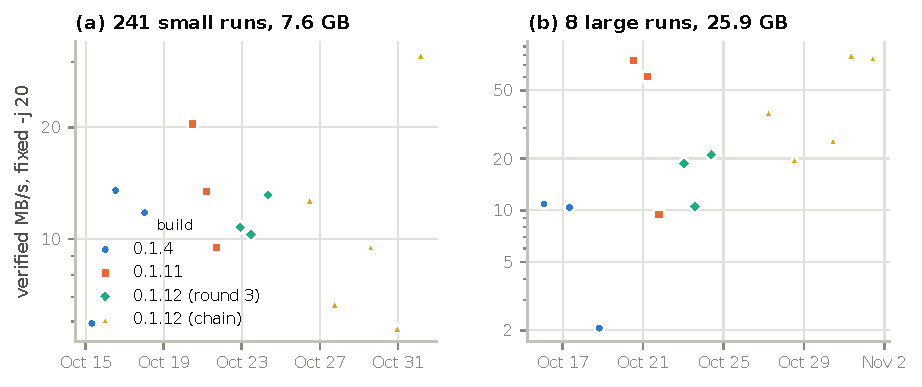
\includegraphics[width=\linewidth]{figs/variability.pdf}
\caption{One configuration over three weeks: adaptiSeq, fixed \code{-j}~20, on D1 (a) and D2 (b), every job that ran it.
Marker shape is the build. The spread is the archive's: the same build on consecutive days differs by up to
fivefold, and the D2 low point (0.1.4, Oct 18) is a run in which ENA served eight corrupt copies.}
\label{fig:variability}
\end{figure}

\begin{figure}[!htb]
\centering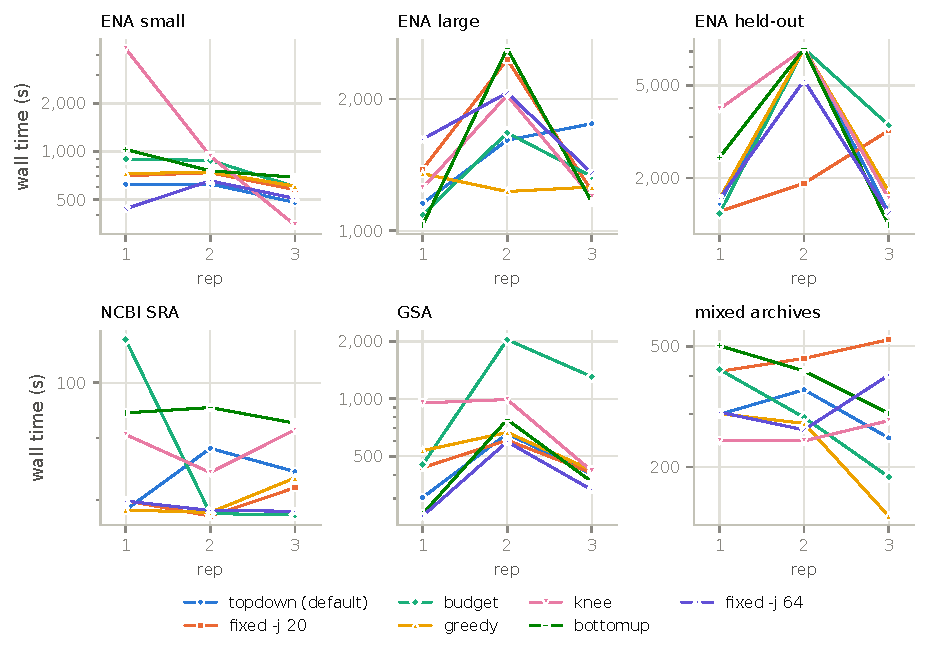
\includegraphics[width=\linewidth]{figs/round3_reps.pdf}
\caption{Round 3 (0.1.12): wall time of each arm in each of three repetitions, per panel. Lines that move together
(4b and 4h rep 2, GSA rep 2) are the archive's hour; lines that cross are differences between arms. Within a panel, the
movement between repetitions is of the same order as the gaps between arms.}
\label{fig:r3reps}
\end{figure}

\subsection{Parallelism is necessary, and its useful level moves}
\label{sec:jsweep}
\figref{fig:jsweep} fixes the number of files in flight and varies it from 1 to 64 (0.1.7, three repetitions). With one
file at a time, D1 took \sweepROne~s and D2 \sweepBOne~s (median). Up to \code{-j}~8, time falls roughly in proportion to \code{-j}
on both lists, as P1 predicts. Beyond it, the curve flattens and becomes noisy: the best median was \code{-j}~\sweepRBestJ{}
on D1 (\sweepRBest~s, \sweepRSpeedup{} times faster than one file at a time) and \code{-j}~\sweepBBestJ{} on D2 (\sweepBBest~s,
\sweepBSpeedup{} times faster), and on D2 \code{-j}~32 lost to both 16 and 64 in all three repetitions because it happened to
settle at ENA's 25-connection ceiling while they reached 50. No single fixed value was best on both lists in all
repetitions, which is the case for a controller (R6). The adaptive default on 0.1.7 sat at \sweepRDefault~s and
\sweepBDefault~s, within 1.4--1.6 times of the best fixed value; later builds changed this (\secref{sec:adaptive}).

\begin{figure}[!htb]
\centering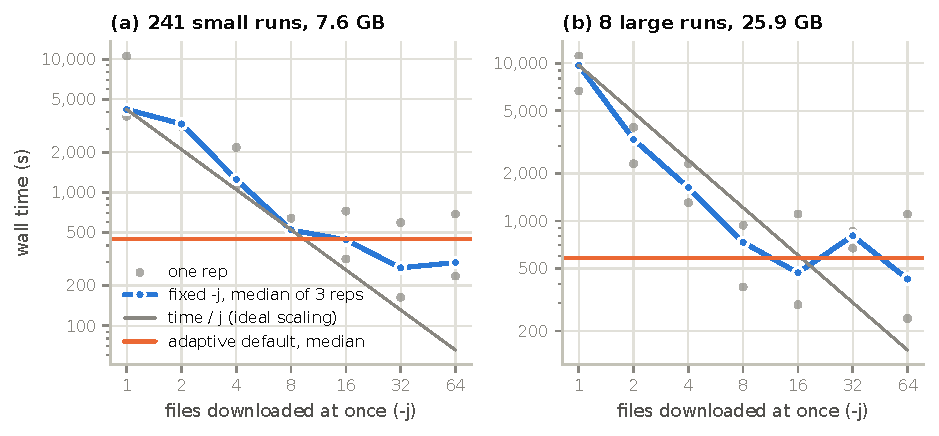
\includegraphics[width=\linewidth]{figs/jsweep.pdf}
\caption{Wall time against the number of files in flight, fixed \code{-j} from 1 to 64 (0.1.7, 3 repetitions; grey dots are
single repetitions, blue the median). The grey line is perfect scaling from \code{-j}~1. The orange line is the adaptive
default's median in the same jobs.}
\label{fig:jsweep}
\end{figure}

\subsection{Keeping connections busy to the end}
\label{sec:tail}
\figref{fig:tail} shows the open archive connections over time for four runs of D2. In 0.1.4 (a, b) the batch moved most
of the 26~GB in the first 25--35 minutes on 18--25 connections, and the run then spent one to two and a half hours on one
to three connections: the tail of each file on one range, and the serial per-run re-download of corrupt files. In 0.1.12
(c, d) the same list held 25 connections until the last minutes and finished in 850 and 1,253~s. \figref{fig:versions}
traces the change across builds on the same panel: the median adaptive-default time fell from \verFirstMed~s (0.1.4) to
\verLastMed~s (0.1.12 chain), and each step lines up with one mechanism of \secref{sec:design}: in-pool md5 and the
ceiling rule (0.1.5: connections rose to 45 where 0.1.4 never passed 25), work stealing (0.1.6), the retried range probe
(0.1.7: no more 1.5~GB files on one connection), and connection-cap recovery (0.1.12).

\begin{figure}[!htb]
\centering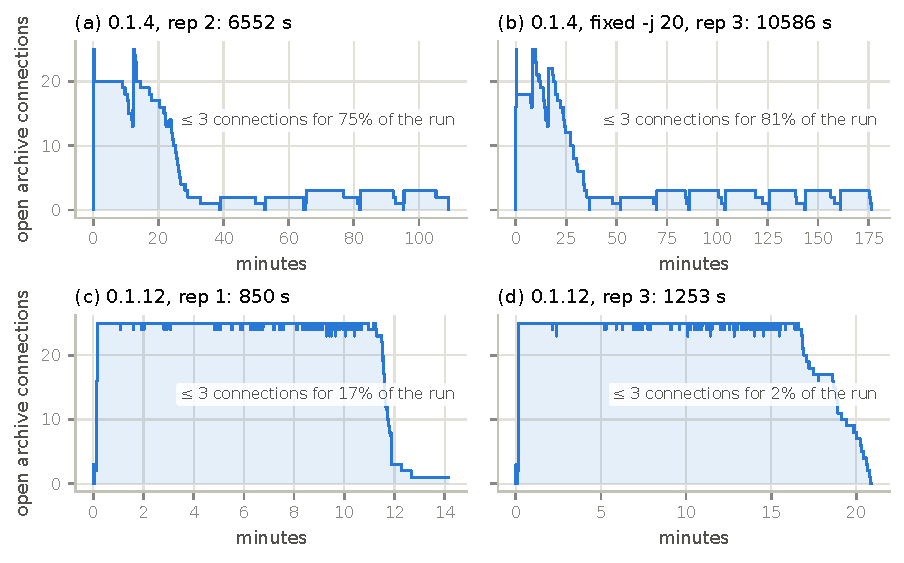
\includegraphics[width=\linewidth]{figs/tail.pdf}
\caption{Open archive connections during four downloads of D2 (8 runs, 25.9~GB). (a, b) Build 0.1.4: after the batch,
the run sat on 1--3 connections for most of its length while corrupt files were re-downloaded one at a time and file
tails ran on single ranges; (b) is the fixed pool, so this is the engine, not the controller. (c, d) Build 0.1.12 on
the same list: 25 connections (ENA's ceiling that day) until the end.}
\label{fig:tail}
\end{figure}

\begin{figure}[!htb]
\centering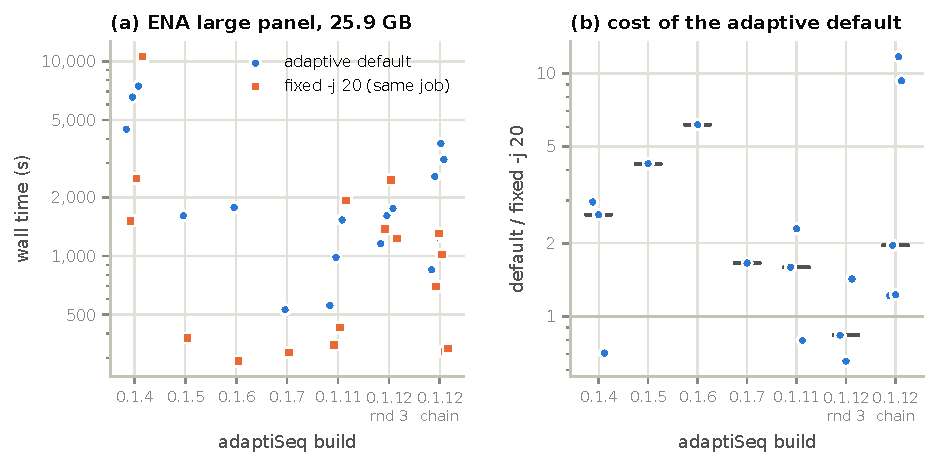
\includegraphics[width=\linewidth]{figs/versions.pdf}
\caption{D2 across builds. (a) Wall time of the adaptive default and of the fixed pool run in the same job. (b) Their
ratio (bars: medians). 0.1.11 and 0.1.12 round 3 are panel 4b of the controller rounds (topdown against fixed \code{-j}~20).
In 0.1.5 and 0.1.6 the engine fixes made the fixed pool fast (288--379~s) while the default was held back by its tail
and by refused range probes; both were fixed in 0.1.6 and 0.1.7.}
\label{fig:versions}
\end{figure}

\subsection{Corrupt copies and in-pool verification}
\label{sec:md5}
\figref{fig:md5} counts md5 mismatches per arm and repetition. Every tool met them; on D2 they appeared in \mdBCases{} of
\mdBRows{} rows, and an affected file costs a full re-download (1.4--1.9~GB on D2, 11.5~GB on 4h). What differs is the
consequence. adaptiSeq deleted each bad copy and fetched it again inside the pool, and in the 0.1.12 chain verified every
run of D2 in all ten adaptiSeq rows. iSeq's first retry re-checks the same file, so its three tries are two downloads;
in rep 2 both iSeq arms gave up on a D2 run after three tries. Kingfisher aborted a whole list on the first corrupt file in
the 0.1.4 run (0 of 8 runs). adaptiSeq missed two distinct D1 runs in the chain. \code{SRR22904330\_1} failed md5 three times
in both adaptiSeq arms' attempts on Oct 27--29 (once as an FTP 550, ``failed to open file'') after every arm had fetched it
cleanly on Oct 26, so ENA's copy was bad or unavailable for days; \code{SRR22904420} failed md5 three times in the default's
rep 5 an hour and a half after the fixed pool had fetched it cleanly. Each was reported in \code{fail.log} with exit status 1.

\begin{figure}[!htb]
\centering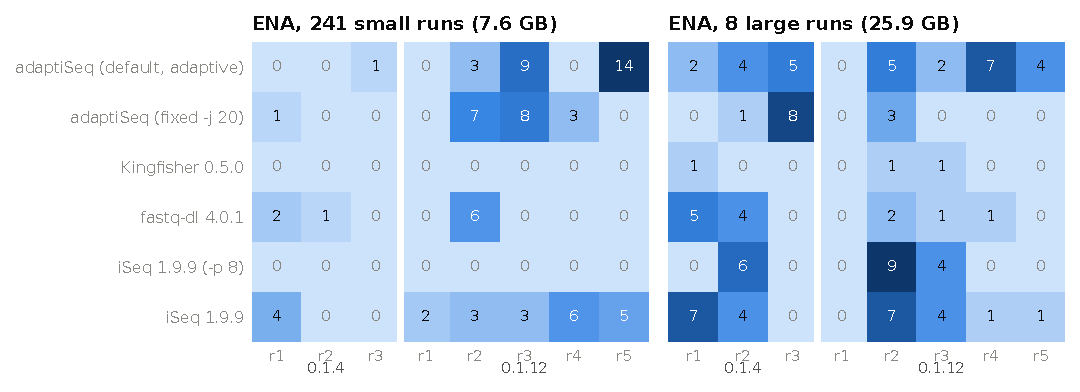
\includegraphics[width=\linewidth]{figs/md5.pdf}
\caption{md5 mismatches logged per arm and repetition, in the 0.1.4 full run (left of each panel) and the 0.1.12 chain
(right). A count is the number of mismatch reports in the arm's log; adaptiSeq reports each failed check, iSeq and
fastq-dl one per retry, Kingfisher one per aborted file. The mismatches move between arms and days: they are bad copies
or bad transfers at the archive, not a property of one tool.}
\label{fig:md5}
\end{figure}

\subsection{Comparison with other tools}
\label{sec:tools}
The final comparison ran five repetitions of both lists on 0.1.12 (\chainStart--\chainEnd).
\figref{fig:chainwall} shows every repetition and \figref{fig:chainratio} every ratio; \tabref{tab:chain} in the appendix
lists all 60 rows.

On D1 (241 small runs), adaptiSeq's fixed pool took a median of \chRFixMed~s (\chRFixMin--\chRFixMax~s) and its default
\chRDefMed~s (\chRDefMin--\chRDefMax~s). The fastest other tool that downloaded every run was, per repetition, a median of
\chRDefVsBestOther{} times slower than the default and \chRFixVsBestOther{} times slower than the fixed pool, and the
other tools hit the 3-hour limit \chRTimeouts{} times. The verified throughput of the other tools' medians never exceeded
\chROtherMBpsMax~MB/s, against \chRDefMBps~MB/s (default) and \chRFixMBps~MB/s (fixed pool).

On D2 (8 large runs), the fixed pool took a median of \chBFixMed~s (\chBFixMin--\chBFixMax~s) at \chBFixMBps~MB/s and the
default \chBDefMed~s (\chBDefMin--\chBDefMax~s). Against the fastest complete other tool per repetition the default was a
median of \chBDefVsBestOther{} times faster, but not always: in repetitions 4 and 5 iSeq with eight \code{axel}
connections finished before the default, which was held back by ENA's 403/416 answers (rep 4) and a fall-back to FTP
(rep 5, \secref{sec:adaptive}). The fixed pool was faster than every other tool that delivered the list, in every
repetition.

The speed comes from R1 and R2: adaptiSeq's default held a median of \chRDefConn{} (D1) and \chBDefConn{} (D2) archive connections,
the single-connection tools one, and iSeq \code{-p 8} up to eight. Because ENA serves each connection at a few MB/s
(P1), connections translate almost directly into throughput.

\begin{figure}[!htb]
\centering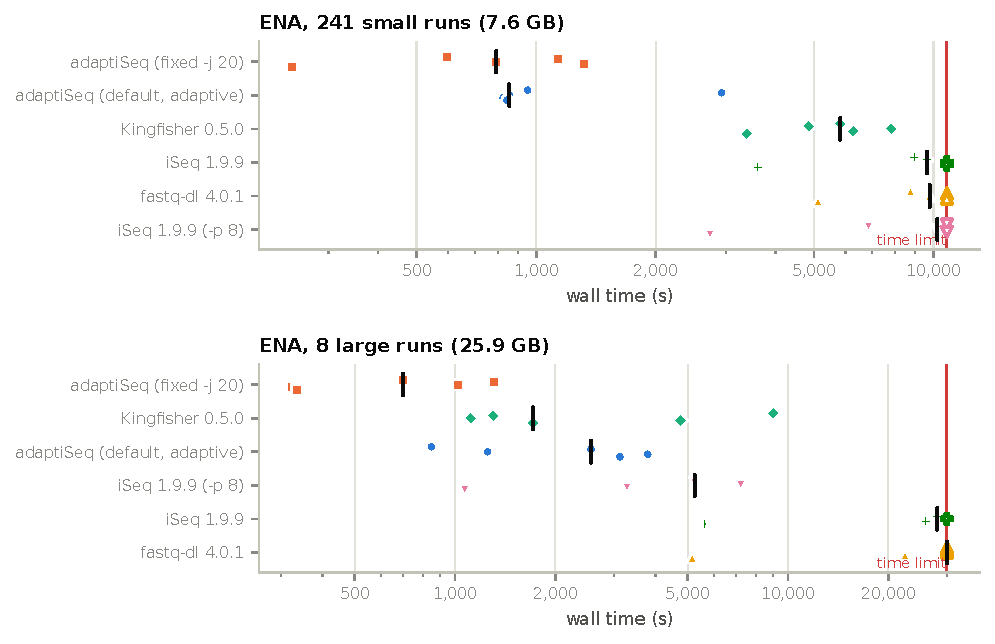
\includegraphics[width=0.9\linewidth]{figs/chain_wall.pdf}
\caption{Wall time of every arm in five repetitions (0.1.12, Oct 26 -- Nov 1). Filled markers finished; hollow markers
hit the time limit (red line) and are lower bounds. Black bars are medians. Arms are ordered by median.}
\label{fig:chainwall}
\end{figure}

\begin{figure}[!htb]
\centering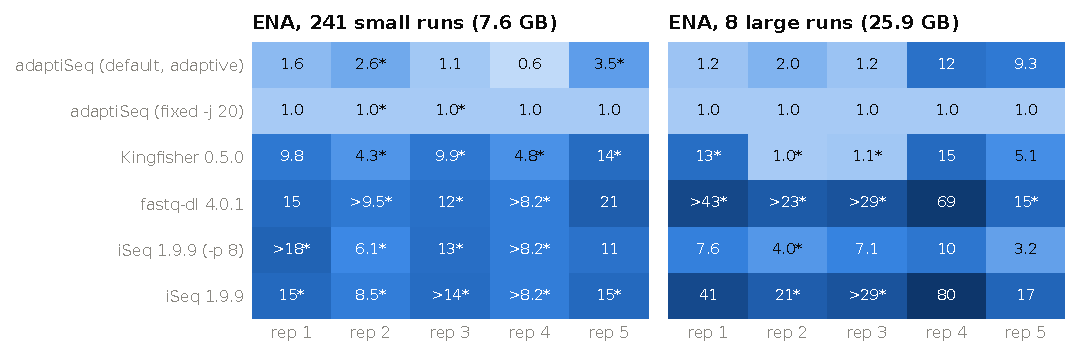
\includegraphics[width=\linewidth]{figs/chain_ratio.pdf}
\caption{Wall time relative to adaptiSeq's fixed pool in the same repetition (darker is slower). ``$>$'' marks a
time limit (lower bound); ``*'' marks a row with fewer than all runs md5-verified, so its time is not for the full list
(Kingfisher's 1.0 on D2 in reps 2 and 3 is a list it abandoned after a few runs).}
\label{fig:chainratio}
\end{figure}

\subsection{Completeness and honest failure}
\label{sec:complete}
\figref{fig:complete} counts, over the five repetitions, how many run downloads each arm delivered md5-verified, delivered
only as unverifiable files, or did not deliver, and how often an arm exited 0 with runs short.

adaptiSeq delivered all runs verified in 16 of its 20 rows. In the other four (D1, one run each; two distinct runs,
\secref{sec:md5}), ENA's copy failed md5 three times or could not be opened, and adaptiSeq exited 1 and named the run in
\code{fail.log}. It never delivered an unverifiable file in the
chain (\chAseqUnverified{} runs) and never exited 0 with a run missing (\chAseqSilent{} of \chAseqRows{} rows).

The other tools exited 0 with runs short in \chOtherSilent{} of their \chOtherRows{} rows, and delivered \chOtherUnverified{}
run downloads as files that cannot be checked against ENA's md5, almost all because ENA's API answered without the FASTQ
columns and the tool silently fetched the run from SRA instead (Kingfisher: 95 runs in rep 5 alone; iSeq: 44). They also
hit the time limit \chOtherTimeouts{} times. For a user, the difference is whether the exit status can be trusted.

\begin{figure}[!htb]
\centering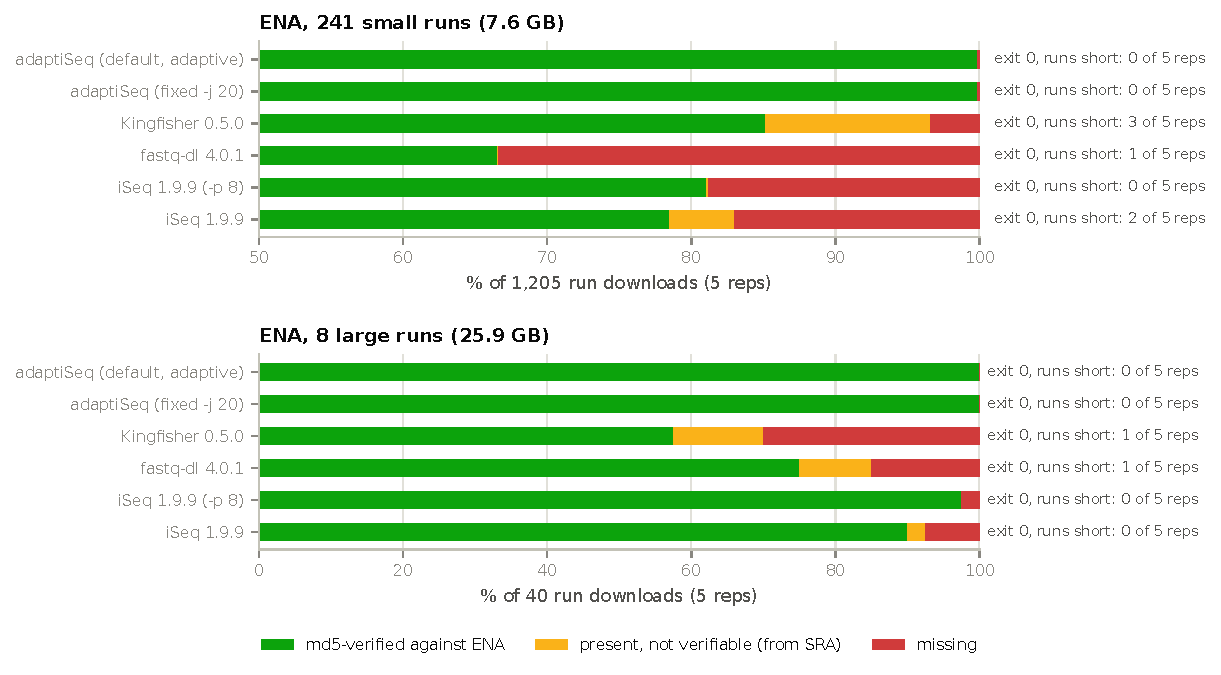
\includegraphics[width=0.92\linewidth]{figs/chain_complete.pdf}
\caption{Run downloads over five repetitions (1,205 on D1, 40 on D2), split into md5-verified, present but not verifiable
against ENA, and missing (including runs not reached before a time limit). Right: repetitions in which the arm exited 0
although runs were short. adaptiSeq's few missing D1 runs all came with exit status 1. The D1 axis starts at 50\%.}
\label{fig:complete}
\end{figure}

\subsection{Controllers across archives}
\label{sec:rounds}
Round 3 ran the five controllers and two fixed pools on six panels from three archives, three repetitions each, on the
final build (\figref{fig:r3heat} and \ref{fig:r3conn}). Three findings:

\begin{enumerate}
\item \textbf{No arm wins everywhere.} Every arm was fastest in at least one case and over 1.5 times the fastest in
another. The archive decides much of it: NCBI (4s) is link-limited, and most arms finish within 25\% of each other; GSA (4g) rewards many connections held through its cut streams; ENA's large files (4b, 4h) are bounded by the
25-connection ceiling and by which arm met a corrupt copy.
\item \textbf{topdown has the best average among the controllers, not overall.} Its mean ratio to the fastest arm was
\rtTdRatio, second to fixed \code{-j}~64 (\rtJsfRatio) and ahead of greedy (\rtGrRatio), fixed \code{-j}~20 (\rtJtwRatio), bottomup
(\rtBoRatio), budget (\rtBuRatio) and knee (\rtKnRatio). Its worst case (\rtTdWorst) was the ENA slow spell on 4h, which
timed out four controllers alike. It was chosen as the default for its average and worst case among the adaptive options.
\item \textbf{Fewer connections cost speed.} knee and budget used the fewest connections (\rtKnConn{} and \rtBuConn{} on
average, \figref{fig:r3conn}) and were the slowest on average; budget remains available for users who want to load the
archive less.
\end{enumerate}

\begin{figure}[!htb]
\centering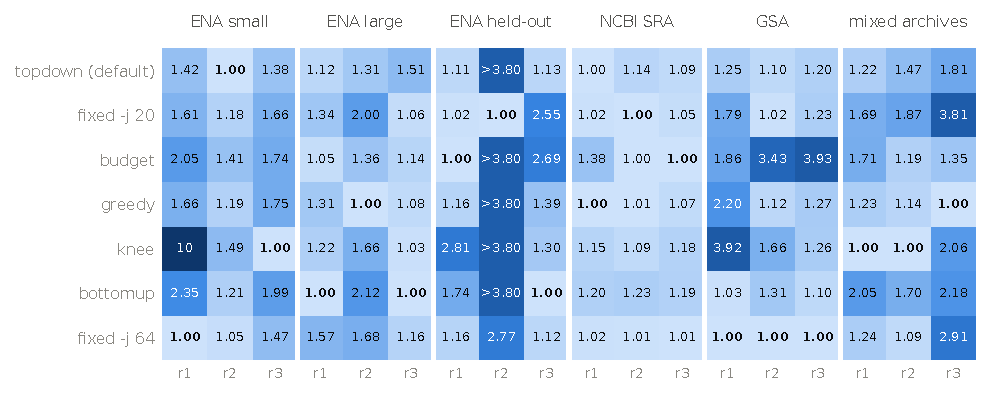
\includegraphics[width=\linewidth]{figs/round3_heat.pdf}
\caption{Round 3 (0.1.12): wall time of each arm over the fastest arm in the same case, for six panels and three
repetitions (bold 1.00 = fastest). ``$>$'' marks a time limit. The 4h rep 2 column is an ENA slow spell: four
controllers ran during it and timed out; fixed \code{-j}~20 ran after it recovered.}
\label{fig:r3heat}
\end{figure}

\begin{figure}[!htb]
\centering
\begin{minipage}{0.52\linewidth}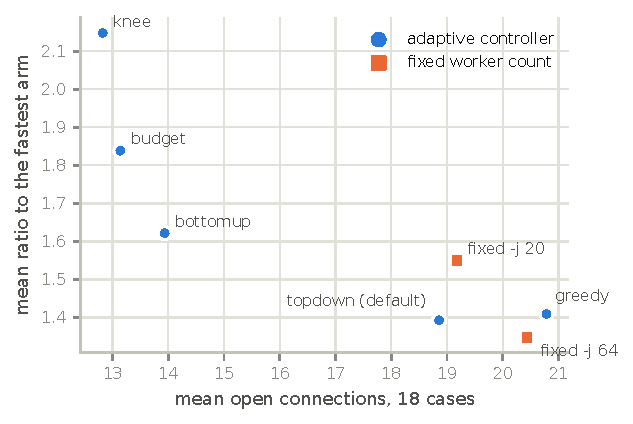
\includegraphics[width=\linewidth]{figs/round3_conn.pdf}\end{minipage}\hfill
\begin{minipage}{0.45\linewidth}\footnotesize\setlength{\tabcolsep}{3.5pt}
\begin{tabular}{@{}lrrrr@{}}
\toprule
Arm & Wins & Worst & Mean & Conn. \\
\midrule
topdown (default) & 3 & 3.80 & 1.39 & 18.9 \\
fixed -j 20 & 7 & 3.81 & 1.55 & 19.2 \\
budget & 4 & 3.93 & 1.84 & 13.1 \\
greedy & 6 & 3.80 & 1.41 & 20.8 \\
knee & 5 & 10.04 & 2.15 & 12.8 \\
bottomup & 4 & 3.80 & 1.62 & 13.9 \\
fixed -j 64 & 9 & 2.91 & 1.35 & 20.4 \\
\bottomrule
\end{tabular}

\end{minipage}
\caption{Round 3 summary over 18 cases. Left: mean open connections against mean ratio to the fastest arm. Right: wins
(within 10\% of the fastest), worst-case ratio, mean ratio, and mean connections. A time limit counts at the limit.}
\label{fig:r3conn}
\end{figure}

\subsection{Where adaptation does not win}
\label{sec:adaptive}
The adaptive default was not the fastest setting. In the five-repetition chain the fixed pool of 20 beat it in 9 of 10
panel-repetitions; the median ratio of default to fixed was \chRDefRatioMed{} on D1 and \chBDefRatioMed{} on D2
(\figref{fig:chainratio}). Three causes stand out in the logs:

\begin{enumerate}
\item \textbf{A failed transport probe.} In rep 2 of D1 and rep 5 of D2 the default's single HTTPS probe failed at the
start, and the cached verdict sent the whole list to segmented FTP, which ENA resets under load. The default then ran at
3.1 and 1.7 mean connections while the fixed pool, a few hours apart, used HTTPS at 15--20 (\figref{fig:ftp}). This is a
transport decision, not a controller decision; re-probing after failures is the obvious fix.
\item \textbf{Range refusals.} In rep 4 of D2, ENA answered 178 range requests with 403 and 29 with 416 during the
default's run; it took 3,789~s, while the fixed pool, which ran later, took 323~s.
\item \textbf{A limit below the controller.} In rep 5 of D1 the default held about 3 connections for the first ten
minutes while the controller held 20 workers, after ENA answered 20 single-connection requests with 403. Something below the
controller held the pool: the per-host cap lowered by those answers, or segments waiting for a connection slot; the default
log level does not show which.
\end{enumerate}

Even so, the adaptive default had properties a fixed value lacks: it was within 1.6 times of the fixed pool in the median
and never needed a value chosen for the list, and on the controller panels its average was within 3\% of the best fixed
pool. The fixed pool's advantage is specific to ENA's present behaviour, where more connections up to the ceiling nearly
always help; on NCBI the extra connections bought nothing (4s), and on GSA the best fixed value changed between repetitions.

\begin{figure}[!htb]
\centering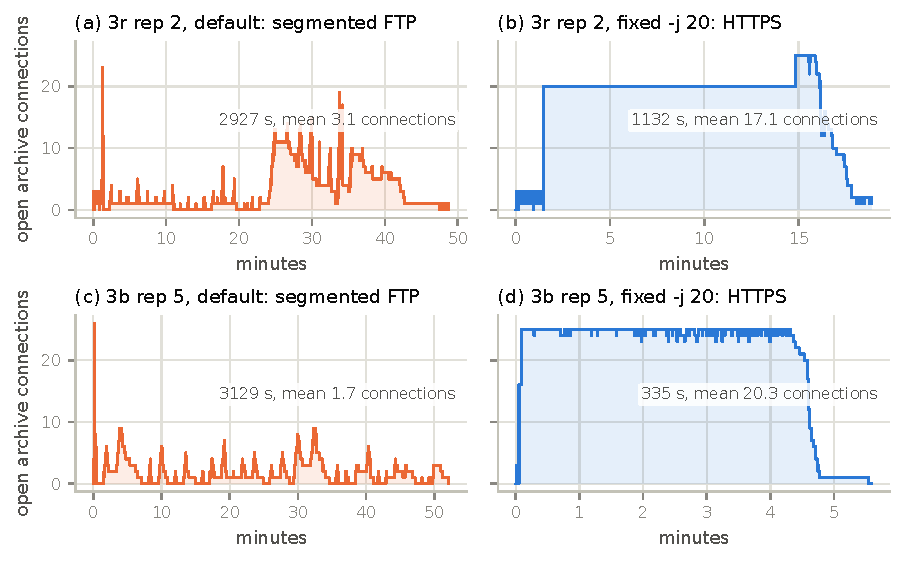
\includegraphics[width=\linewidth]{figs/ftp_fallback.pdf}
\caption{Open archive connections for the default and the fixed pool in two repetitions where the default's HTTPS probe
failed and it used segmented FTP for the whole list. The fixed pool ran in the same job, earlier.}
\label{fig:ftp}
\end{figure}

\subsection{Threats to validity}
\begin{itemize}
\item \textbf{Archive state.} The largest source of variance is the archive (\secref{sec:noise}). Paired ratios, repeated
runs over days, and reporting every repetition reduce but do not remove it; a different week could reorder close arms.
\item \textbf{One site.} All results are from Expanse's network. Per-connection rates elsewhere differ (a FABRIC node saw
1.0--1.2~MB/s per ENA connection, within Expanse's range); the per-connection behaviour of P1 was the same.
\item \textbf{Builds.} The campaigns span builds 0.1.4 to 0.1.12; cross-build comparisons (\figref{fig:versions},
\ref{fig:variability}) mix design changes with archive changes. The tool comparison and the controller round each use one
build.
\item \textbf{Sequential arms.} Arms in a repetition ran hours apart on 3b (single-connection tools take up to 8~hours),
so pairing within a repetition shares the day, not the minute.
\item \textbf{Counting.} md5 mismatch counts come from log lines whose wording differs between tools. Connections are
sampled at 5~Hz and miss very short-lived connections.
\item \textbf{Time limits} make the slow tools' times lower bounds; their true ratios are larger than shown.
\end{itemize}

%=====================================================================
\section{Summary}
%=====================================================================
Downloading public sequencing data is limited by the archive, not the client's link: ENA serves each connection at a few
MB/s, its API fails for hours, it serves corrupt copies, and it refuses connections past a moving ceiling. adaptiSeq's design
answers each of these: many connections across and within files, kept busy to the last byte; refusals read as a ceiling;
every file checked as it lands and re-fetched in parallel; and no silent substitution or skipping. On ENA lists of small and
large runs it was several times faster than iSeq, Kingfisher and fastq-dl in every repetition, and it was the only tool whose
exit status always matched what it delivered. Its adaptive default is a reasonable no-tuning setting rather than the fastest
one: a fixed pool of 20 was faster on most ENA cases, and every number here depends on the state of ENA's and NCBI's servers
during the run.

\begin{thebibliography}{9}\small
\bibitem{iseq} Chao H, Li Z, Chen D, Chen M. iSeq: an integrated tool to fetch public sequencing data.
\emph{Bioinformatics}, 2024, btae641. doi:10.1093/bioinformatics/btae641.
\bibitem{fastbiodl} Swargo RM, Arslan E, Arifuzzaman M. Adaptive parallel downloader for large genomic datasets.
arXiv:2508.05511, 2025.
\bibitem{kingfisher} Woodcroft BJ et al. Kingfisher: download and extraction of sequence data and metadata.
\url{https://github.com/wwood/kingfisher-download}, version 0.5.0.
\bibitem{fastqdl} Petit RA III, Read TD. fastq-dl: download FASTQ files from ENA or SRA.
\url{https://github.com/rpetit3/fastq-dl}, version 4.0.1.
\end{thebibliography}

\appendix
\section{All rows of the five-repetition comparison}
\small
\setlength{\tabcolsep}{4pt}
\begin{longtable}{@{}lllrrlrrrr@{}}
\caption{Every row of the 0.1.12 chain. Ratio: wall time over fixed \code{-j}~20 in the same repetition. Runs: md5-verified of expected, (+N) present but unverified. Exit: 0, non-zero code, or ``limit''. MB/s: md5-verified bytes over wall time. Conn.: mean/max archive connections. md5: mismatch reports in the log.}
\label{tab:chain}\\
\toprule
Panel & Rep & Arm & Wall (s) & Ratio & Runs & Exit & MB/s & Conn. & md5 \\
\midrule
\endfirsthead
\toprule
Panel & Rep & Arm & Wall (s) & Ratio & Runs & Exit & MB/s & Conn. & md5 \\
\midrule
\endhead
3r & 1 & adaptiSeq \code{-j} 20 & 596 & 1.00 & 241/241 & 0 & 12.73 & 15.6/25 & 0 \\
3r & 1 & adaptiSeq default & 952 & 1.60 & 241/241 & 0 & 7.97 & 20.1/25 & 0 \\
3r & 1 & Kingfisher & 5,825 & 9.77 & 241/241 & 0 & 1.30 & 2.1/5 & 0 \\
3r & 1 & fastq-dl & 8,742 & 14.67 & 241/241 & 0 & 0.87 & 1.0/1 & 0 \\
3r & 1 & iSeq & 8,951 & 15.02 & 233/241 (+8) & 0 & 0.77 & 1.0/1 & 2 \\
3r & 1 & iSeq \code{-p} 8 & 10,800 & >18.12 & 37/241 (+1) & limit & 0.40 & 4.7/8 & 0 \\
\midrule
3r & 2 & adaptiSeq \code{-j} 20 & 1,132 & 1.00 & 240/241 & 1 & 6.69 & 17.1/25 & 7 \\
3r & 2 & adaptiSeq default & 2,927 & 2.59 & 240/241 & 1 & 2.59 & 3.1/23 & 3 \\
3r & 2 & Kingfisher & 4,856 & 4.29 & 233/241 (+8) & 0 & 1.29 & 1.7/5 & 0 \\
3r & 2 & iSeq \code{-p} 8 & 6,852 & 6.05 & 239/241 & 1 & 1.11 & 3.9/8 & 0 \\
3r & 2 & iSeq & 9,628 & 8.50 & 239/241 (+1) & 1 & 0.79 & 1.0/1 & 3 \\
3r & 2 & fastq-dl & 10,800 & >9.54 & 43/241 & limit & 0.54 & 1.0/1 & 6 \\
\midrule
3r & 3 & adaptiSeq \code{-j} 20 & 794 & 1.00 & 240/241 & 1 & 9.54 & 14.2/25 & 8 \\
3r & 3 & adaptiSeq default & 855 & 1.08 & 241/241 & 0 & 8.87 & 16.5/25 & 9 \\
3r & 3 & Kingfisher & 7,835 & 9.87 & 240/241 (+1) & 0 & 0.97 & 1.7/5 & 0 \\
3r & 3 & fastq-dl & 9,778 & 12.32 & 240/241 & 0 & 0.78 & 1.0/1 & 0 \\
3r & 3 & iSeq \code{-p} 8 & 10,223 & 12.88 & 240/241 & 1 & 0.74 & 3.6/8 & 0 \\
3r & 3 & iSeq & 10,800 & >13.61 & 103/241 & limit & 0.61 & 1.0/1 & 3 \\
\midrule
3r & 4 & adaptiSeq default & 826 & 0.63 & 241/241 & 0 & 9.19 & 15.6/33 & 0 \\
3r & 4 & adaptiSeq \code{-j} 20 & 1,317 & 1.00 & 241/241 & 0 & 5.76 & 18.3/25 & 3 \\
3r & 4 & Kingfisher & 6,276 & 4.76 & 166/241 (+34) & 1 & 0.77 & 1.4/5 & 0 \\
3r & 4 & iSeq & 10,800 & >8.20 & 174/241 (+1) & limit & 0.66 & 1.0/1 & 6 \\
3r & 4 & fastq-dl & 10,800 & >8.20 & 37/241 (+1) & limit & 0.40 & 1.0/1 & 0 \\
3r & 4 & iSeq \code{-p} 8 & 10,800 & >8.20 & 220/241 & limit & 0.70 & 4.1/8 & 0 \\
\midrule
3r & 5 & adaptiSeq \code{-j} 20 & 242 & 1.00 & 241/241 & 0 & 31.29 & 15.2/25 & 0 \\
3r & 5 & adaptiSeq default & 844 & 3.48 & 240/241 & 1 & 8.98 & 5.9/25 & 14 \\
3r & 5 & iSeq \code{-p} 8 & 2,738 & 11.30 & 241/241 & 0 & 2.77 & 3.3/8 & 0 \\
3r & 5 & Kingfisher & 3,386 & 13.97 & 146/241 (+95) & 0 & 2.09 & 1.7/5 & 0 \\
3r & 5 & iSeq & 3,608 & 14.89 & 197/241 (+44) & 0 & 1.16 & 0.8/1 & 5 \\
3r & 5 & fastq-dl & 5,117 & 21.11 & 241/241 & 0 & 1.48 & 0.9/1 & 0 \\
\midrule
3b & 1 & adaptiSeq \code{-j} 20 & 699 & 1.00 & 8/8 & 0 & 37.03 & 22.1/25 & 0 \\
3b & 1 & adaptiSeq default & 850 & 1.22 & 8/8 & 0 & 30.43 & 20.5/25 & 0 \\
3b & 1 & iSeq \code{-p} 8 & 5,288 & 7.57 & 8/8 & 0 & 4.89 & 5.6/8 & 0 \\
3b & 1 & Kingfisher & 9,039 & 12.94 & 5/8 (+3) & 0 & 1.56 & 2.0/5 & 0 \\
3b & 1 & iSeq & 28,310 & 40.52 & 8/8 & 0 & 0.91 & 1.0/1 & 0 \\
3b & 1 & fastq-dl & 30,000 & >42.94 & 6/8 (+1) & limit & 0.60 & 1.0/1 & 0 \\
\midrule
3b & 2 & Kingfisher & 1,302 & 1.00 & 2/8 (+1) & 1 & 5.46 & 4.0/5 & 1 \\
3b & 2 & adaptiSeq \code{-j} 20 & 1,307 & 1.00 & 8/8 & 0 & 19.80 & 23.8/25 & 3 \\
3b & 2 & adaptiSeq default & 2,561 & 1.96 & 8/8 & 0 & 10.10 & 27.8/50 & 5 \\
3b & 2 & iSeq \code{-p} 8 & 5,245 & 4.01 & 7/8 & 1 & 4.21 & 6.4/8 & 9 \\
3b & 2 & iSeq & 28,053 & 21.47 & 7/8 & 1 & 0.81 & 1.0/1 & 7 \\
3b & 2 & fastq-dl & 30,000 & >22.96 & 5/8 (+1) & limit & 0.53 & 1.0/1 & 2 \\
\midrule
3b & 3 & adaptiSeq \code{-j} 20 & 1,020 & 1.00 & 8/8 & 0 & 25.36 & 24.0/25 & 0 \\
3b & 3 & Kingfisher & 1,115 & 1.09 & 0/8 (+1) & 1 & 1.19 & 4.3/5 & 1 \\
3b & 3 & adaptiSeq default & 1,253 & 1.23 & 8/8 & 0 & 20.64 & 22.3/25 & 2 \\
3b & 3 & iSeq \code{-p} 8 & 7,208 & 7.07 & 8/8 & 0 & 3.59 & 7.3/8 & 4 \\
3b & 3 & iSeq & 30,000 & >29.41 & 5/8 (+1) & limit & 0.47 & 1.0/1 & 4 \\
3b & 3 & fastq-dl & 30,000 & >29.41 & 4/8 (+1) & limit & 0.42 & 1.0/1 & 1 \\
\midrule
3b & 4 & adaptiSeq \code{-j} 20 & 323 & 1.00 & 8/8 & 0 & 80.05 & 41.5/50 & 0 \\
3b & 4 & iSeq \code{-p} 8 & 3,286 & 10.16 & 8/8 & 0 & 7.87 & 6.1/8 & 0 \\
3b & 4 & adaptiSeq default & 3,789 & 11.72 & 8/8 & 0 & 6.83 & 21.7/49 & 7 \\
3b & 4 & Kingfisher & 4,759 & 14.72 & 8/8 & 0 & 5.44 & 4.0/5 & 0 \\
3b & 4 & fastq-dl & 22,446 & 69.44 & 8/8 & 0 & 1.15 & 1.0/1 & 1 \\
3b & 4 & iSeq & 25,890 & 80.09 & 8/8 & 0 & 1.00 & 1.0/1 & 1 \\
\midrule
3b & 5 & adaptiSeq \code{-j} 20 & 335 & 1.00 & 8/8 & 0 & 77.13 & 20.3/25 & 0 \\
3b & 5 & iSeq \code{-p} 8 & 1,071 & 3.19 & 8/8 & 0 & 24.17 & 5.0/8 & 0 \\
3b & 5 & Kingfisher & 1,715 & 5.11 & 8/8 & 0 & 15.08 & 2.8/5 & 0 \\
3b & 5 & adaptiSeq default & 3,129 & 9.33 & 8/8 & 0 & 8.27 & 1.7/26 & 4 \\
3b & 5 & fastq-dl & 5,154 & 15.36 & 7/8 (+1) & 0 & 4.24 & 1.0/26 & 0 \\
3b & 5 & iSeq & 5,625 & 16.77 & 8/8 & 0 & 4.60 & 1.0/1 & 1 \\
\bottomrule
\end{longtable}


\end{document}
